%%%%%%% Lecture Notes Style for Concrete Mathematics %%%%%%%%%%%%%
%%%%%%% Taught by Patrick White, TJHSST %%%%%%%%%%%%%%%%%%%%%%%%%%

\documentclass[11pt,twosided]{article}
%%%%%%%%%%%%%%%%%%%%%%%%%%%%%%%%%%%%%%%%%%%%%%%%%%%%%%%
%%%% HEADER FILE for CONCRETE MATH LECTURE NOTES %%%%%%
%%%%%%%%%%%%%%%%%%%%%%%%%%%%%%%%%%%%%%%%%%%%%%%%%%%%%%%

%%%%%%%%%%%%%%%%%%%%%%%%%%%%%%%%%%%%%%%%%%%%%%%%%%%%%%%%%%%%%%%%%%%
%% This file is included at the top of every lecture notes file %%%
%% It should ONLY be changed by the instructor %%
%%%%%%%%%%%%%%%%%%%%%%%%%%%%%%%%%%%%%%%%%%%%%%%%%%%%%%%%%%%%%%%%%%%

%%%%%%%%%%%%%%%%%%%%%% package inclusions %%%%%%%%%%%%%%%%%%%%
%\usepackage[
%top=2cm,
%bottom=2cm,
%left=3cm,
%right=2cm,
%headheight=17pt, % as per the warning by fancyhdr
%includehead,includefoot,
%heightrounded, % to avoid spurious underfull messages
%]{geometry} 


\usepackage{amsmath,amssymb,amsfonts}
\usepackage{longtable}
\usepackage{mathtools}
\usepackage{amsthm}
\usepackage{enumerate}
\usepackage{fancyhdr}
\pagestyle{fancy}


%%%%%%%%%%%%%%% theorem style definitions %%%%%%%%%%%%%%%%%%%%%%
\newtheorem{theorem}{Theorem}[section]
%\newtheorem{corollary}{Corollary}[theorem]
%\newtheorem{lemma}[theorem]{Lemma}
\newtheorem*{remark}{Remark}
%\newtheorem{example}{Example}[section]
\newtheorem*{definition}{Definition}


%%%%%%%%%%%%%%%% custom function definitions %%%%%%%%%%%%%%%%%%%%%%%%%
%%%%%%%%%%% as class progresses, this section may be enhanced %%%%%%%%

\def\multiset#1#2{\ensuremath{\left(\kern-.3em\left(\genfrac{}{}{0pt}{}{#1}{#2}\right)
		\kern-.3em\right)}} %%% multiset notation
\newcommand\rf[2]{{#1}^{\overline{#2}}} %%%% rising factorial \rf{x}{m}
\newcommand\ff[2]{{#1}^{\underline{#2}}} %%%%% falling factorial \ff{x}{m}
\newcommand{\Perm}[2]{{}^{#1}\!P_{#2}} % permutation
\newcommand{\half}{\ensuremath{\frac{1}{2}}}
\newcommand{\braces}[1]{\left\{#1\right\}}
\newcommand{\set}[1]{\braces{#1}}
\newcommand{\snb}[2]{\ensuremath{\left(\kern-.3em\left(\genfrac{}{}{0pt}{}{#1}{#2}\right)\kern-.3em\right)}}
\newcommand{\fallingfactorial}[1]{^{\underline{#1}}}
\newcommand{\fallfac}[2]{{#1}^{\underline{#2}}}
\newcommand{\stirlingone}[2]{\genfrac[]{0pt}{1}{#1}{#2}}
\newcommand{\stiri}[2]{\stirlingone{#1}{#2}}
\newcommand{\dstirlingone}[2]{\genfrac[]{0pt}{0}{#1}{#2}}
\newcommand{\dstiri}[2]{\dstirlingone{#1}{#2}}
\newcommand{\stirlingtwo}[2]{\genfrac\{\}{0pt}{1}{#1}{#2}}
\newcommand{\stirii}[2]{\stirlingtwo{#1}{#2}}
\newcommand{\dstirlingtwo}[2]{\genfrac\{\}{0pt}{0}{#1}{#2}}
\newcommand{\dstirii}[2]{\dstirlingtwo{#1}{#2}}
\newcommand{\ol}[1]{\overline{#1}}
%%%%%%%
% book stuff
%%%%%%%%%

\usepackage[twoside,outer=1.5in,inner=2in,bottom=1.5in,top=1.5in,marginpar=2in]{geometry} 
\usepackage{scrextend}
\usepackage{palatino}
\usepackage{multicol}
\usepackage{float}
\usepackage[hidelinks]{hyperref}
\usepackage[nameinlink, capitalise, noabbrev]{cleveref}
%\usepackage{background}
\usepackage{graphicx}
\usepackage{listliketab}

\usepackage{lipsum}
\usepackage{caption}
\usepackage{marginnote}

\reversemarginpar


\usepackage[dvipsnames]{xcolor}
\usepackage{amsthm}
\usepackage{shadethm}

\setlength{\parindent}{0pt}

\newcommand*\Note{%
	\marginnote[\textcolor{blue}{\raggedright{\LARGE ?}\ Note }]{}%
}
\newcommand*\Warn{%
	\marginnote[\textcolor{red}{\raggedright{\LARGE !}\ Warning }]{}%
}
\reversemarginpar

\newcommand{\N}{\mathbb{N}}
\newcommand{\Z}{\mathbb{Z}}
\newcommand{\I}{\mathbb{I}}
\newcommand{\R}{\mathbb{R}}
\newcommand{\Q}{\mathbb{Q}}
\renewcommand{\qed}{\hfill$\blacksquare$}
\let\newproof\proof
\renewenvironment{proof}{\begin{addmargin}[1em]{0em}\begin{newproof}}{\end{newproof}\end{addmargin}\qed}
% \newcommand{\expl}[1]{\text{\hfill[#1]}$}


\newenvironment{lemma}[2][Lemma]{\begin{trivlist}
		\item[\hskip \labelsep {\bfseries #1}\hskip \labelsep {\bfseries #2.}]}{\end{trivlist}}
\newenvironment{problem}[2][Problem]{\begin{trivlist}
		\item[\hskip \labelsep {\bfseries #1}\hskip \labelsep {\bfseries #2.}]}{\end{trivlist}}
\newenvironment{example}[2][Example]{\begin{trivlist}
		\item[\hskip \labelsep {\bfseries #1}\hskip \labelsep{\bfseries #2.}]}{\end{trivlist}}
\newenvironment{solution}{{\noindent \bfseries Solution\hskip 2ex}}{\qed}
\newenvironment{exercise}[2][Exercise]{\begin{trivlist}
		\item[\hskip \labelsep {\bfseries #1}\hskip \labelsep {\bfseries #2.}]}{\end{trivlist}}
\newenvironment{reflection}[2][Reflection]{\begin{trivlist}
		\item[\hskip \labelsep {\bfseries #1}\hskip \labelsep {\bfseries #2.}]}{\end{trivlist}}
\newenvironment{proposition}[2][Proposition]{\begin{trivlist}
		\item[\hskip \labelsep {\bfseries #1}\hskip \labelsep {\bfseries #2.}]}{\end{trivlist}}
\newenvironment{corollary}[2][Corollary]{\begin{trivlist}
		\item[\hskip \labelsep {\bfseries #1}\hskip \labelsep {\bfseries #2.}]}{\end{trivlist}}

%%%% add package inclusions here, if any
\usepackage{blubase}
%%%%% Define your custom functions and macros here, if any

%%%%%%%%%%%%%%%%%%%% Define the variables below %%%%%%%%%%%%%%%%%%%%%%%%%%%%%%
\def\titlestring{The Calkin-Wilf Tree}
\def\scribestring{Bryan Lu}
\def\datestring{Thursday, April 4, 2019}


%%%%%%%%%%%%%%%%%%% Page Headers -- Do Not Change %%%%%%%%%%%%%%%%%%%%%%%%%%%
\lhead{\titlestring}
\rhead{Page \thepage}
\cfoot{Concrete Math -- White -- TJHSST}
\renewcommand{\headrulewidth}{0.4pt}
\renewcommand{\footrulewidth}{0.4pt}

%%%%%%%%%%%%%%%%% Begin the document %%%%%%%%%%%%%%%%%%%%%%%%%
\begin{document}
\thispagestyle{plain}  %% no headers on this page

%%%% Do not change these lines %%%%%
\noindent
{\LARGE \textbf{\titlestring}}\\\\
%
{\Large Scribe: \scribestring}\\ \\
{\textbf{Date}: \datestring}


%%%%%%%%%%%%%%%%%%%%%%%%%% YOUR CONTENT GOES HERE %%%%%%%%%%%%%%%%%%%%%%%%%%
\noindent

\section{The Calkin-Wilf Tree}
\begin{problem}{1}
What is the 23rd rational positive number? 	
\end{problem}
\begin{solution}
	We don't know - we need an ordering. 
\end{solution}

We will introduce the \textbf{hyperbinary} numbers to do this. Numbers are written in the same way as traditional binary, but we allow 2s as digits. 

\begin{problem}{2}
How many ways are there to write $n$ in hyperbinary, $b(n)$? 
\end{problem}
\begin{solution}
	We will construct a recurrence as follows. Consider if the number $n$ is even or odd. If we have the odd integer $2n+1$, we must have 1 as its last digit. If we lop off the 1, the number of ways to write $2n+1$ in hyperbinary is clearly the number of ways to write $n$ in hyperbinary. Thus, $b(2n+1) = b(n)$. 	
This gives us the recurrence relations 
\[
	b(2n+1) = b(n) \quad b(2n+2) = b(n+1) + b(n)
\]	
\end{solution}

Now, if we consider the sequence $\left\{\frac{b(n)}{b(n+1)}\right\}_{n=0}^\infty$, we claim that this sequence contains every rational in reduced form exactly once. 

To show this, we consider constructing a complete binary tree such that if we run a breadth-first search on this tree, we would get this sequence in order. Here is a rendering of this tree for clarity:

\begin{center}
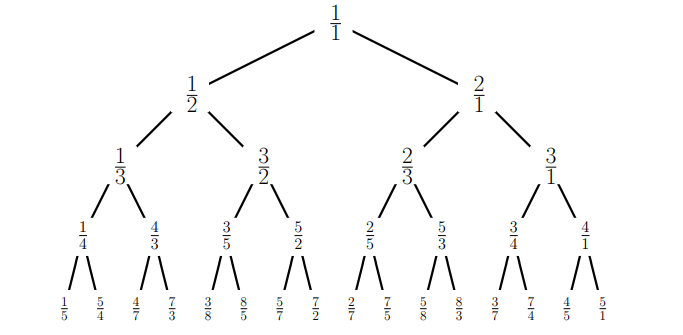
\includegraphics[scale=0.9]{calkinwilf.png}\\
\end{center}

Notice that by construction, the node with the number $\frac{b(n)}{b(n+1)}$ has the child $\frac{b(2n+1)}{b(2n+2)}$ to the left and the child $\frac{b(2n+2)}{b(2n+3)}$ to the right. From our recurrence relation, we have that these are equal to $\frac{b(n)}{b(n) + b(n+1)}$ and $\frac{b(n) + b(n+1)}{b(n+1)}$, respectively.

Therefore, for a node with the value $\frac{N}{D}$, it has the child $\frac{N}{N+D}$ to the left and the child $\frac{N+D}{D}$ to the right. We can show similarly that the parent of the node $\frac{x}{y}$ is $\frac{x}{y-x}$ if $y > x$ or $\frac{x-y}{y}$ if $x > y$. 

With this structure in mind, we will prove the three following claims by contradiction. 


\textbf{Claim 1.} $\gcd(x, y) = 1$ if $ \frac{x}{y} \in T$, $\frac{x}{y} \neq 1$. 
\begin{proof}
	Assume by contradiction there exists some $\frac{x}{y}$ in the tree such that $\gcd(x, y) = k$ and without loss of generality $\frac{x}{y} = \frac{kx'}{ky'}$ is the node with the closest distance to the root. The parent of this node therefore either must be $\frac{kx'}{k(y'-x')}$ or $\frac{k(x'-y')}{ky'}$, but then the numerator and denominator have a common factor at least $k$, contradiction. Thus all $\frac{x}{y}$ in the tree are in lowest terms. 	
\end{proof}

\textbf{Claim 2.} If $\frac{x}{y} \in \ZZ$ and $\gcd(x, y) = 1$, $ \frac{x}{y} \in T$. 
\begin{proof}
Suppose by contradiction we can construct the set $S$ of all rationals not in the tree. Let $y$ be the minimum of the all the denominators in $S$, and $x$ be the lowest numerator of all the numbers not in the tree that have the  denominator $y$. Thus, $\frac{x}{y}$ can be said to be the "smallest" number not in the tree. 

If $x > y$, then we can consider the number $\frac{x-y}{y}$. This can't be in the tree because its child $\frac{x}{y}$ is not in the tree. However, $x-y < x$, so $\frac{x}{y}$ is not the "smallest" member of the set $S$, contradiction. 

Similarly, if $x < y$, we consider the number $\frac{x}{y-x}$, which can't be in the tree either, but $y- x < y$, contradiction. 

Therefore, all rational numbers appear at least once in the tree. 
\end{proof}

\textbf{Claim 3.} All rationals $\frac{x}{y}$, $x, y \in \ZZ$ appear exactly once $\frac{x}{y} \in T$. 
\begin{proof}
Suppose by contradiction we can construct the set of $S$ of all rationals that appear at least twice. By a similar method in the last proof, we take the "smallest" number in $S$. When considering the parent of this number in the tree, we note that this can either be $\frac{x}{y-x}$ or $\frac{x-y}{y}$, which must also appear at least twice. However, $x - y < x$ and $y - x < y$, so these parents are "smaller" than $\frac{x}{y}$, which is a contradiction. 
\end{proof}

This gives us the following theorem now: 
\begin{theorem}
The sequence $\left\{\frac{b(n)}{b(n+1)}\right\}_{n=0}^\infty$ includes every rational number exactly once in lowest terms. 
\end{theorem}

A cool way to find the $n$th number in this sequence - consider writing $n$ in (regular) binary, running a run-length encoding of the binary string backwards (omitting the actual digits), and then constructing the continued fraction. This works very nicely :) - here is solution to our original problem by this ordering: 

\[
 23 = 10111_2 \rightarrow \text{run-length encoding: } 311
\]

\[
\implies 3 + \frac{1}{1 + \frac{1}{1}} = 3 + \frac{1}{2} = \frac{7}{2}
\]

\end{document}
